
\chead{Principal Component Analysis}
%\input{tcilatex}

\begin{document}

\tableofcontents
%http://support.sas.com/publishing/pubcat/chaps/55129.pdf

\section{Introduction to Course}
Advances in data collection and storage capabilities during the past decades have led to an information
overload in most sciences. Researchers working in domains as diverse as engineering, astronomy, biology,
remote sensing, economics, and consumer transactions, face larger and larger observations and simulations
on a daily basis.

Such datasets, in contrast with smaller, more traditional datasets that have been studied
extensively in the past, present new challenges in data analysis. Traditional statistical methods break down
partly because of the increase in the number of observations, but mostly because of the increase in the
number of variables associated with each observation. The dimension of the data is the number of variables
that are measured on each observation.\\(I Fodor, LLNL, USA, June 2002).

\section{Overview of Course}

To ground the students in Applied Multivariate Analysis. This module serves business and mathematics students. It introduces the mathematical statistical ideas behind \begin{itemize} \item Principal Component Analysis, \item Factor Analysis, \item Cluster Analysis, \item Discrimination Function, \item The Multiple Linear Logistic function. \end{itemize}
The students learn how to implement these techniques in SPSS to become competent in the analysis of a wide variety of multivariate data structures.
%%%%%%%%%%%%%%%%%%%%%%%%%%%%%%%%%%%%%%%%%%%%%%%%%%%%%%%%%%%%%%%%%%%%%%%
\section{Data Reduction}
\begin{itemize}
\item Data Reduction or Dimensionality Reduction pertains to analytic methods (typically multivariate exploratory techniques such as Factor Analysis, Multidimensional Scaling, Cluster Analysis, Canonical Correlation, or Neural Networks) that involve reducing the dimensionality of a data set by extracting a number of underlying factors, dimensions, clusters, etc., that can account for the variability in the (multidimensional) data set.

\item For example, in poorly designed questionnaires, all responses provided by the participants on a large number of variables (scales, questions, or dimensions) could be explained by a very limited number of "trivial" or artifactual factors. For example, two such underlying factors could be: (1) the respondent's attitude towards the study (positive or negative) and (2) the "social desirability" factor (a response bias representing a tendency to respond in a socially desirable manner).
\end{itemize}
%%%%%%%%%%%%%%%%%%%%%%%%%%%%%%%%%%%%%%%%%%%%%%%%%%%%%%%%%%%%%%%%%%%%%%%
\subsection{Variable Redundancy}
A specific (but fictitious) example of research will now be presented to illustrate the concept of
variable redundancy introduced earlier. Imagine that you have developed a 7-item measure of
job satisfaction. The \emph{instrument} is reproduced here:


\begin{framed}
\begin{verbatim}
Please respond to each of the following statements by placing a
rating in the space to the left of the statement. In making your
ratings, use any number from 1 to 7 in which 1=“strongly disagree”
and 7=“strongly agree.”
_____ 1. My supervisor treats me with consideration.
_____ 2. My supervisor consults me concerning important decisions
that affect my work.
_____ 3. My supervisors give me recognition when I do a good job.
_____ 4. My supervisor gives me the support I need to do my job
well.
_____ 5. My pay is fair.
_____ 6. My pay is appropriate, given the amount of responsibility
that comes with my job.
_____ 7. My pay is comparable to the pay earned by other employees
whose jobs are similar to mine.
\end{verbatim}
\end{framed}

Notice that items 1-4 all deal with the same topic: the employees’ satisfaction with their supervisors. In this way, items 1-4 are somewhat redundant to one another. Similarly, notice that items 5-7 also all seem to deal
with the same topic: the employees’ satisfaction with their pay. Empirical findings may further support the notion that there is redundancy in the seven items. Assume that you administer the questionnaire to 200 employees and compute all possible correlations between responses to the 7 items. The resulting fictitious correlations are
reproduced in the table below.

\begin{figure}
	\centering
	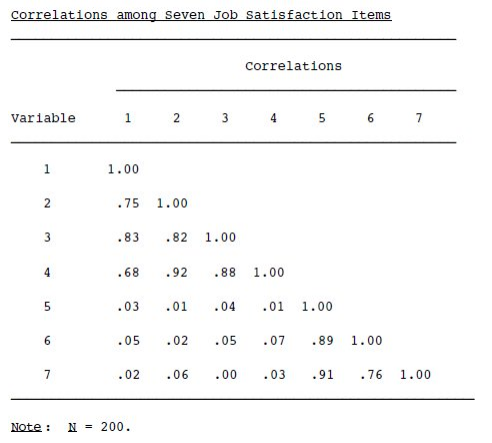
\includegraphics[width=0.7\linewidth]{3Acorrelation}
	\caption{}
	\label{fig:3acorrelation}
\end{figure}


When correlations among several variables are computed, they are typically summarized in the
form of a correlation matrix, such as the one reproduced in the previous table. This is an appropriate
opportunity to review just how a correlation matrix is interpreted.

The rows and columns of the table correspond to the seven variables included in the analysis: Row 1 (and column 1)
represents variable 1, row 2 (and column 2) represents variable 2, and so forth. Where a given
row and column intersect, you will find the correlation between the two corresponding variables.
For example, where the row for variable 2 intersects with the column for variable 1, you find a
correlation of 0.75; this means that the correlation between variables 1 and 2 is 0.75.
The correlations show that the seven items seem to hang together in two distinct
groups.

First, notice that items 1-4 show relatively strong correlations with one another. This
could be because items 1-4 are measuring the same construct. In the same way, items 5-7
correlate strongly with one another (a possible indication that they all measure the same
construct as well). Even more interesting, notice that items 1-4 demonstrate very weak
correlations with items 5-7. This is what you would expect to see if items 1-4 and items 5-7
were measuring two different constructs.

Given this apparent redundancy, it is likely that the seven items of the questionnaire are not
really measuring seven different constructs; more likely, items 1-4 are measuring a single
construct that could reasonably be labelled \textbf{\emph{satisfaction with supervision}} while items 5-7 are
measuring a different construct that could be labelled \textbf{\emph{satisfaction with pay}}.

If responses to the seven items actually displayed the redundancy suggested by the pattern of
correlations, it would be advantageous to somehow reduce the number of variables
in this data set, so that (in a sense) items 1-4 are collapsed into a single new variable that reflects
the employees’ satisfaction with supervision, and items 5-7 are collapsed into a single new
variable that reflects satisfaction with pay.

We could then use these two new artificial variables (rather than the seven original variables) as predictor variables in multiple regression, or in any other type of analysis.

In essence, this is what is accomplished by principal component analysis: it allows you to reduce
a set of observed variables into a smaller set of artificial variables called principal components.
The resulting principal components may then be used in subsequent analyses.
\newpage
\subsection{Data Reduction in Exploratory Graphics}

The term can also refer in \textbf{exploratory graphics} to ``Data Reduction by unbiased decreasing of the sample size". This type of Data Reduction is applied in exploratory graphical data analysis of extremely large data sets. The size of the data set can obscure an existing pattern (especially in large line graphs or scatterplots) due to the density of markers or lines. Then, it can be useful to plot only a representative subset of the data (so that the pattern is not hidden by the number of point markers) to reveal the otherwise obscured but still reliable pattern.

\section{Principal Component Analysis }

\subsection{Introduction}
\begin{itemize}
	\item Principal component analysis is appropriate when you have obtained measures on a number of
	(possibly) correlated observed variables and wish to develop a smaller number of artificial uncorrelated variables called \textbf{principal components} that will account for most of the variance in the observed variables. The first principal component accounts for as much of the variability in the data as possible, and each succeeding component accounts for as much of the remaining variability as possible. The principal
	components may then be used as predictor or criterion variables in subsequent analyses.
	
	
\item Traditionally, principal component analysis is performed can be performed on raw data, on the symmetric \textbf{Covariance matrix} or on the symmetric \textbf{Correlation matrix}. (The covariance matrix contains scaled sums of squares and cross products. A correlation matrix is like a covariance matrix but first the variables, i.e. the columns, have been standardized.)
	
\item If raw data is used, the procedure will create the original correlation matrix or covariance matrix, as specified by the user.  If the correlation matrix is used, the variables are standardized and the total variance will equal the number of variables used in the analysis (because each standardized variable has a variance equal to 1).  If the covariance matrix is used, the variables will remain in their original metric. 
\item  However, one must take care to use variables whose variances and scales are similar.  Unlike \textbf{factor analysis}, which analyzes the common variance, the original matrix in a principal components analysis analyzes the total variance.  Also, principal components analysis assumes that each original measure is collected without measurement error.
\end{itemize}






\subsection{Mathematical background of PCA}
Principal Component Analysis is a linear \textbf{dimensionality reduction} technique, which identifies orthogonal directions of maximum variance in the original data, and projects the data into a lower-dimensionality space formed of a sub-set of the highest-variance components (Bishop, 1995).


The mathematical technique used in PCA is called \textbf{eigen analysis}. Technically, a principal component can be
defined as a linear combination of optimally-weighted observed variables. Software packages compute solutions for these weights by using a special
type of equation called an \textbf{\emph{eigenequation}}. The weights produced by these eigenequations are
optimal weights in the sense that, for a given set of data, no other set of weights could produce a
set of components that are more successful in accounting for variance in the observed variables.
The weights are created so as to satisfy a principle of least squares that is similar (but not identical) to
the principle of least squares used in multiple regression.

Remarks
\begin{itemize}
	\item The words \textbf{\emph{linear combination}} refer to the fact that scores on a
	component are created by adding together scores on the observed variables being analyzed.
	\item \textbf{\emph{Optimally weighted}} refers to the fact that the observed variables are weighted in such a way
	that the resulting components account for a maximal amount of variance in the data set.
\end{itemize}

%We solve for the eigenvalues and eigenvectors of a square symmetric matrix with sums of squares and cross products. The eigenvector associated with the largest eigenvalue has the same direction as the first principal component. Similarly the eigenvector associated with the second largest eigenvalue determines the direction of the second principal component, and so on. The sum of the eigenvalues equals the \textbf{trace} of the square matrix and the maximum number of eigenvectors equals the number of rows (or columns) of this matrix.

\subsection{Number of Extracted Components}
\begin{itemize}
	\item The preceding section may have created the impression
	that, if a principal component analysis were performed on data from the 7-item job satisfaction
	questionnaire, only two components would be created.  However, such an impression would not
	be entirely correct.
	
\item In reality, the number of components extracted in a principal component analysis \textbf{\emph{is equal}} to the
	number of observed variables being analyzed.  This means that an analysis of your 7-item
	questionnaire would actually result in seven components, not two.
	
\item 	However, in most analyses, only the first few components account for meaningful amounts of
	variance, so only these first few components are retained, interpreted, and used in subsequent
	analyses (such as in multiple regression analyses).  
	
\item For example, in your analysis of the 7-item
	job satisfaction questionnaire, it is likely that only the first two components would account for a
	meaningful amount of variance; therefore only these would be retained for interpretation.  You
	would assume that the remaining five components accounted for only trivial amounts of
	variance.  These latter components would therefore not be retained, interpreted, or further
	analyzed.
\end{itemize}

\subsection{Characteristics of Principal Components}
\begin{itemize}
	\item The first component extracted in a principal component analysis accounts for a maximal amount of total variance in the observed variables. Under typical conditions, this means that the first component will be correlated with at least
	some of the observed variables.  In fact it may be correlated with many.
	
\item The second component extracted will have two important characteristics.  First,  this component
	will account for a maximal amount of variance in the data set that was not accounted for by the
	first component.  Again under typical conditions, this means that the second component will be
	correlated with some of the observed variables that did not display strong correlations with
	component 1.
\item The second characteristic of the second component is that it will be uncorrelated with the first
	component. If you were to compute the correlation between components 1 and 2, that
	correlation should be close to zero.
	
\item The remaining components that are extracted in the analysis display the same two characteristics:
	each component accounts for a maximal amount of variance in the observed variables that was
	not accounted for by the preceding components, and is uncorrelated with all of the preceding
	components.  
	\item A principal component analysis proceeds in this fashion, with each new component
	accounting for progressively smaller and smaller amounts of variance (this is why only the first
	few components are usually retained and interpreted).  When the analysis is complete, the
	resulting components will display varying degrees of correlation with the observed variables, but
	are completely uncorrelated with one another.
\end{itemize}


\subsection{Total Variance in the context of PCA}
To understand the meaning of \textbf{total
	variance} as it is used in a principal component analysis, remember that the observed
variables are standardized in the course of the analysis.  This means that each variable is
transformed so that it has a mean of zero and a variance of one.

The total variance in the
data set is simply the sum of the variances of these observed variables.  Because they have
been standardized to have a variance of one, each observed variable contributes one unit of
variance to the total variance in the data set.  Because of this, the total variance in a
principal component analysis \textbf{\emph{will always be equal}} to the number of observed variables
being analyzed.

For example, if seven variables are being analyzed, the total variance will
equal seven.  The components that are extracted in the analysis will partition this variance:
perhaps the first component will account for 3.2 units of total variance; perhaps the second
component will account for 2.1 units.  The analysis continues in this way until all of the
variance in the data set (i.e. the remaining 1.7 units). has been accounted for.

\subsection{Orthogonal versus Oblique Solutions}

This course will discuss only principal component analysis that result in \textbf{orthogonal solutions}.
An orthogonal solution is one in which the components remain uncorrelated (orthogonal means
“uncorrelated”).

It is possible to perform a principal component analysis that results in correlated components.
Such a solution is called an \textbf{oblique solution}.  In some situations, oblique solutions are superior
to orthogonal solutions because they produce cleaner, more easily-interpreted results.
However, oblique solutions are also somewhat more complicated to interpret, compared to
orthogonal solutions.  For this reason, we will focus only on the interpretation of orthogonal solutions


\end{document} 
